\documentclass{article}
\usepackage[a4paper, margin=1in]{geometry}
\usepackage{graphicx}
\usepackage{setspace}
\usepackage{ctex}
\usepackage{enumitem}

\begin{document}

\begin{center}
    \vspace*{3cm} % 控制顶部空白
    {\Huge 《数据库系统原理》大作业 \\[1cm]}
    {\LARGE 系统设计报告 \\[5cm]}
\end{center}

\begin{center}
    {\Large 题目名称:航医通} \\[4cm]
\end{center}

\begin{center}
    \begin{tabular}{ll}
        {\Large 学号及姓名:} & {\Large \underline{22371056 孟烜宇(组长)}} \\[0.5cm]
        & {\Large \underline{22373040 余欣实}} \\[0.5cm]
        & {\Large \underline{22371328 曹玮琳}} \\[3cm]
    \end{tabular}
\end{center}

\begin{center}
    {\Large 2024\hspace{0.35cm} 年 \hspace{0.35cm} 10\hspace{0.35cm} 月 \hspace{0.35cm} 4\hspace{0.35cm} 日}
\end{center}

\newpage

\begin{center}
    \vspace*{3cm}
    \LARGE 组内同学承担任务说明
\end{center}

\vspace{2.5cm}

\begin{center}
\renewcommand{\arraystretch}{3} % 调整行高
\setlength{\tabcolsep}{10pt} % 调整列间距
\small % 调整字体大小
\begin{tabular}{|c|p{2cm}|p{2cm}|p{2cm}|c|}
    \hline
    \textbf{学生姓名} & \multicolumn{3}{c|}{\textbf{工作内容}} & \textbf{工作量占比} \\ 
    \cline{2-4}
     & \textbf{子任务 1:系统功能设计与数据库设计} & \textbf{子任务 2:系统服务器端开发} & \textbf{子任务 3:系统客户端开发} & \textbf{(组内同学总和为 1)} \\
    \hline
    孟烜宇& & & & \\
    \hline
    余欣实& & & & \\
    \hline
    曹玮琳& & & & \\
    \hline
\end{tabular}
\end{center}

\newpage

\tableofcontents

\newpage

\section{需求分析}
\subsection{需求描述}
\subsubsection{背景调研}

社会发展不停歇,人们对于医疗服务的需求也在不断增加。在这种情况下,医疗服务的质量和效率也成为了人们关注的焦点。
与此同时,大学生作为国家的希望与未来,其身体健康状况引起了社会的广泛关注。但是,大学生的健康却不容乐观。诸如“脆皮大学生”等问题愈演愈烈,睡眠质量不足、饮食不规律、容易受伤等问题困扰着许多大学生。
大学如何担起培养社会主义现代化强国的建设者和接班人的伟大使命?
高校医疗健康体系如何在中华民族伟大复兴战略全局和世界百年未有之大变局中,顺应潮流把握机遇,面临挑战?
为祖国培养“健康工作七十年的红色工程师”的北京航空航天大学,应当以怎样的技术和平台来保证学生的医疗健康呢?
这些问题值得我们深思。

首先,必须认识到校园医疗服务的多元性,涵盖从日常健康管理到突发疾病的应急处理。
这种多元性意味着校园医疗服务不仅要提供基础的医疗诊断和治疗,还需要针对不同疾病类型和健康问题提供个性化的解决方案,以满足学生的各种需求。通过全面的服务体系,能够更有效地应对学生在学习和生活中可能遇到的健康挑战。

其次,通过构建一个集成化的医疗服务平台,不仅能够提升学生的就医体验,还能为学校的整体健康教育提供数据支持和决策依据。
该平台可以集中管理学生的健康档案、就医记录和预约信息,使得医疗服务更加高效和便捷。同时,汇总的数据可以帮助学校分析学生的健康趋势,识别常见健康问题,从而制定更具针对性的健康教育方案和预防措施,以提高整体校园健康水平。

但是,北京航空航天大学目前缺少这么一个完善的医疗服务网络平台。学生在体检、就医等过程中程序繁琐,信息不对称,导致就医效率低下,学校也无法全面了解学生的健康状况。

因此,本团队希望开发一个功能强大且集成,数据安全的医疗服务平台,以提升学生的就医体验,提高学校的医疗服务水平。
这就是航医通开发的初衷。

\subsubsection{用户画像}
校园医疗服务平台的主要用户有以下几类:

\begin{itemize}[itemsep=0.01em]
    \item 在读学生
    \item 教职工
    \item 医护人员
    \item 管理人员
\end{itemize}

初步用户画像侧写如下:

\begin{figure}[h]
    \centering
    % 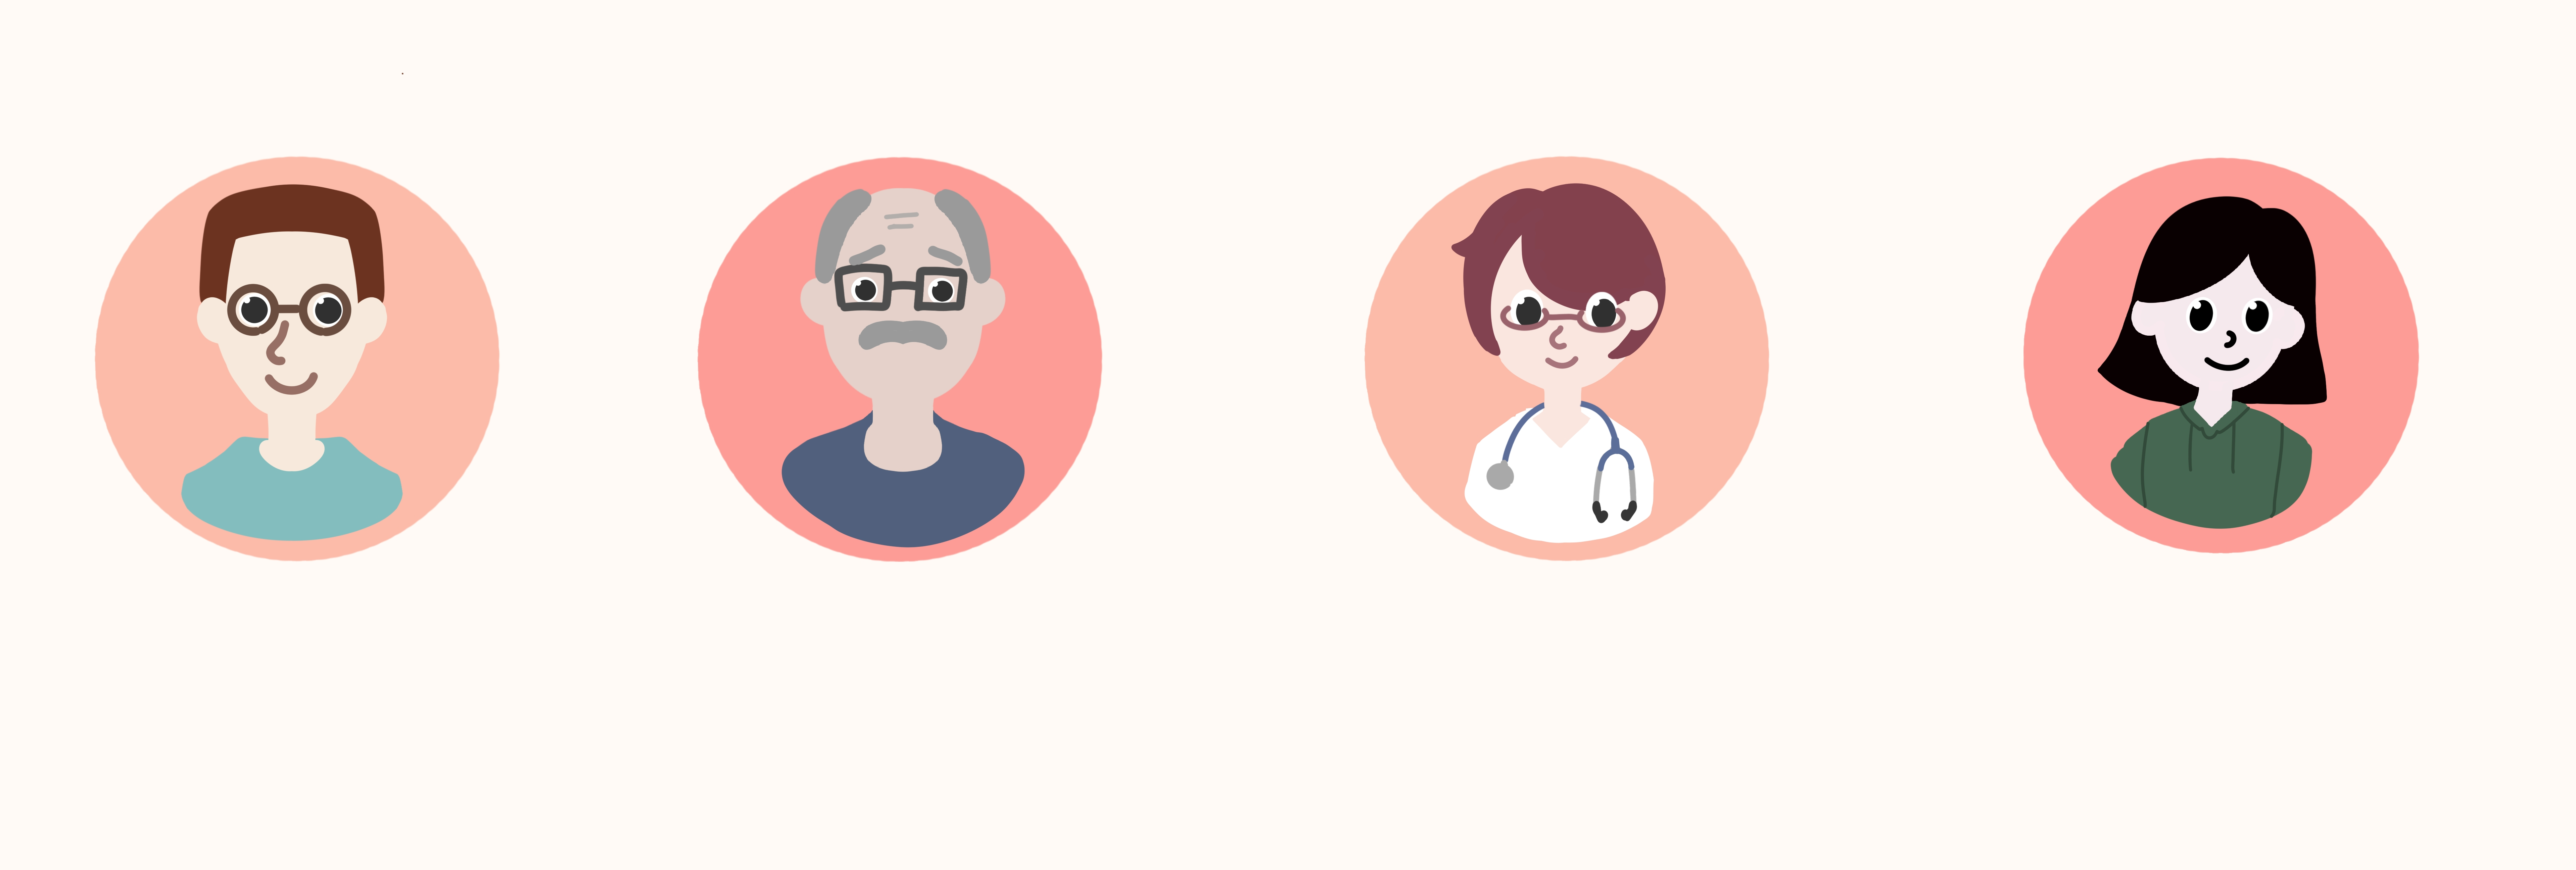
\includegraphics[width=0.8\textwidth]{images/user.png}
    \caption{用户画像}
\end{figure}

\subsubsection{需求分析}

经过上述背景调研和用户画像的分析,我们可以总结出需求如下:
\vspace{0.5cm}

对于每一位在读学生,我们希望能够提供以下服务:
\begin{enumerate}[itemsep=0.01em]
    \item 拥有在线上查看医生排班并为自己\textbf{预约挂号}权限,能够选择合适时间段就诊。
    \item 能够查看自己的排队信息,\textbf{候诊查询}。
    \item 能够线上进行\textbf{在线缴费},包括挂号费、药费等。
    \item 能够在线购买一些非处方药品,\textbf{在线购药}。
    \item 对于每年的体检,能够在线上选择体检时间和项目,\textbf{预约体检}。
    \item 可以对于就诊经历进行评价,提供\textbf{医生评价}功能。
    \item 能够查看自己的\textbf{健康档案},包括体检记录、病历、就诊记录、处方等。
    \item 可以进行\textbf{在线健康咨询}。
    \item 能够接受相关\textbf{通知提醒},如体检提醒、就诊提醒等。
    \item 定期接受\textbf{健康讲座},提供健康教育。
\end{enumerate}

\vspace{0.5cm}
对于教职工,我们希望能够提供以下服务:
\begin{enumerate}[itemsep=0.01em]
    \item 拥有在线上查看医生排班并为自己和家人\textbf{预约挂号}权限,能够选择合适时间段就诊。
    \item 能够查看自己的排队信息,\textbf{候诊查询}。
    \item 能够线上进行\textbf{在线缴费},包括挂号费、药费等。
    \item 能够在线购买一些非处方药品,\textbf{在线购药}。
    \item 可以对于就诊经历进行评价,提供\textbf{医生评价}功能。
    \item 能够查看自己的\textbf{健康档案},包括体检记录、病历、就诊记录、处方等。
    \item 可以进行\textbf{在线健康咨询}。
    \item 能够接受相关\textbf{通知提醒},如体检提醒、就诊提醒等。
\end{enumerate}

\vspace{0.5cm}
对于医护人员,我们希望能够提供以下服务:
\begin{enumerate}[itemsep=0.01em]
    \item 能够查看自己的\textbf{排班信息}。
    \item 可以查看预约记录,\textbf{预约查询}。
    \item 可以查看排队信息,\textbf{候诊查询}。
    \item 可以查看\textbf{患者信息},包括病历、就诊记录、处方等。
    \item 能够进行\textbf{在线诊断},并进行回复。
    \item 可以查看\textbf{患者评价},并进行回复。
    \item 能够接受相关\textbf{通知提醒},如排班提醒、患者评价提醒等。
    \item 能够创建或者更新\textbf{患者病历}。
    \item 可以开具处方并记录药品信息,\textbf{处方管理}。
\end{enumerate}

\vspace{0.5cm}
对于管理人员,我们希望能够提供以下服务:
\begin{enumerate}[itemsep=0.01em]
    \item 能够查看\textbf{医疗数据分析},包括患者病历统计、疾病统计等。
    \item 可以查看并管理\textbf{医疗服务评价}。
    \item 能够进行\textbf{医疗排班},添加、修改或删除医生的排班信息。
    \item 可以管理药品信息和库存,\textbf{药品管理}。
    \item 查看和管理预约记录,\textbf{预约管理}。
\end{enumerate}

\vspace{0.5cm}
另外对于\textbf{数据库管理员}:
\begin{enumerate}[itemsep=0.01em]
    \item 具有管理用户的权限,可以检索,修改,增加,删除所有的用户信息。
    \item 具有管理预约的权限,可以检索,修改,增加,删除所有的预约信息。
    \item 具有管理药品、处方、病历等信息的权限。
\end{enumerate}

\subsection{数据流图}
% 在此处添加数据流图

\subsection{数据元素表}

% 在此处添加数据元素表

\section{数据库概念模式设计}
\subsection{系统初步E-R 图}
% 在此处添加系统初步E-R 图

\subsection{系统基本 E-R 图}
% 在此处添加系统基本 E-R 图

\section{数据库逻辑模式设计与优化}
\subsection{数据库关系模式定义}
% 在此处添加由 E-R 图得到的关系模式

\subsection{关系模式范式等级的判定与规范化}
% 在此处添加关系模式范式等级的判定与规范化内容,注:要规范到 3NF

\subsection{数据库关系模式优化}
% 在此处添加数据库关系模式优化内容

\section{数据库物理设计}
% 在此处说明所选择的存取方法,给出索引定义

\end{document}
